\documentclass{article}
\usepackage{graphicx}
\usepackage{polski}
\usepackage{enumerate}

\title{Lista 2}
\author{Maciej Kmieciak, 277516}
\date{11.2024}

\begin{document}

\maketitle

\section{Wstęp}

Zaimplementowałem algorytmy: Quick Sort z modyfikacją polegającą na dzieleniu na trzy części; Radix Sort względem dowolnej podstawy \texttt{d}; implementację Insertion Sort na liście (stworzonej jako własna struktura) oraz Bucket Sort z modyfikacją, która daje działania dla dowolnych liczb (a nie tylko z przedziału \((0, 1]\). Porównałem działanie Radix Sort dla różnych podstaw, a także Quick Sort z Bucket Sort.

\section{Najciekawsze fragmenty kodu}

Poniżej znajdują się kluczowe fragmenty zmodyfikowanych wersji algorytmów. Tutaj usunąłem z nich liczniki porównań i przypisań.

\subsection{Modyfikacja Quick Sort}

\begin{verbatim}
array<int, 2> partition_mod(int A[], int p, int k) {
    if (A[p] > A[k]) {
        swap(A[p], A[k]);
    }
    int leftPivot = A[p];
    int rightPivot = A[k];

    int i = p + 1,
        j = p + 1,
        g = k - 1;

    while (j <= g) {
        if (A[j] < leftPivot) {
            swap(A[i], A[j]);
            ++i;
        }
        else if (A[j] > rightPivot) {
            while (A[g] > rightPivot && j < g) {
                --g;
            }
            
            swap(A[j], A[g]);
            --g;

            if (A[j] < leftPivot) {
                swap(A[i], A[j]);
                ++i;
            }
        }
        ++j;
    }
    
    --i;
    ++g;
    swap(A[p], A[i]);
    swap(A[k], A[g]);

    return { i, g };
}
\end{verbatim}

To zmodyfikowana funkcja \texttt{partition}. Indeks \texttt{i} przechowuje pozycję, na którą powienien trafić następny element mniejszy od \texttt{leftPivot}. \texttt{j} przechodzi przez tablicę z lewa na prawo. \texttt{g} przechowuje pozycję, na którą ma trafić następny element większy od \texttt{rightPivot}. Przechodząc przez tablicę zamieniamy elementy odpowiednio, jeśli trzeba, tzn. przerzucamy je na lewo od lewego pivota, na prawo od prawego lub pozostawiamy na "środku", jeśli liczba jest pomiędzy wartościami pivotów. Na koniec wstawiamy same pivoty we właściwe miejsca i zwracamy ich indeksy.

\subsection{Modyfikacja Radix Sort}

\begin{verbatim}
void radix(int A[], int d) {
    int max_val = A[0];

    for (int i = 1; i < n; ++i) {
        if (A[i] > max_val) {
            max_val = A[i];
        }
    }

    int num_digits = log(max_val) / log(d) + 1;

    int digit_place = 1;
    for (int i = 0; i < num_digits; ++i) {
        counting(A, digit_place, d);
        digit_place *= d;
    }
}

void counting(int A[], int digit_place, int d) {
    int* C = new int[d]();
    int* B = new int[n];   

    for (int i = 0; i < n; ++i) {
        int digit = (A[i] / digit_place) % d;
        ++C[digit];
    }

    for (int j = 1; j < d; ++j) {
        C[j] += C[j - 1];
    }

    for (int i = n - 1; i >= 0; --i) {
        int digit = (A[i] / digit_place) % d;
        B[C[digit] - 1] = A[i];
        --C[digit];
    }

    for (int i = 0; i < n; ++i) {
        A[i] = B[i];
    }
}
\end{verbatim}

Najpierw szukamy maksimum, żeby potem określić liczbę cyfr do posortowania z użyciem logarytmu o podstawie \texttt{d}. Następnie, dla każdej cyfry-miejsca, zaczynając od najmniej znaczącej, wykonujemy procedurę \texttt{counting}. Wewnątrz niej, wydobywamy cyfrę na danym miejscu dla każdej liczby z tablicy. Tworzymy "pudełka" odpowiadające kolejnym cyfrom i umieszczcamy tam liczbę, która ma daną cyfrę na danym miejscu. Następnie przepisujemy liczby z powrotem do oryginalnej tablicy, w kolejności od najmniejszej cyfry (na danym miejscu) do największej i przechodzimy do kolejnej, bardziej znaczącej cyfry-miejsca.

\subsection{Insertion Sort zaimplementowane na liście}

\begin{verbatim}
void insert(Node** sorted, Node* newNode) {
    if (!*sorted || (*sorted)->data >= newNode->data) {
        newNode->next = *sorted;
        *sorted = newNode;
    }
    else {
        Node* current = *sorted;
        while (current->next && current->next->data < newNode->data) {
            current = current->next;
        }
        newNode->next = current->next;
        current->next = newNode;
    }
}
\end{verbatim}

Powyżej znajduje się procedura \texttt{insert}, która wstawia nowy element do posortowanej listy, zgodnie z zasadą działania Insertion Sort. Przesuwamy się po kolejnych elementach listy, zaczynając od najmniejszego tak długo, jak element do wstawienia jest od nich mniejszy. Następnie wstawiamy nowy element pomiędzy ostatni, który był mniejszy a jego następcę.

\subsection{Modyfikacja Bucket Sort}

\begin{verbatim}
float* bucket_mod(const float* unsorted) {
	float* A = new float[n];

	for (int i = 0; i < n; ++i) {
		A[i] = unsorted[i];
	}

	float min_val = A[0], max_val = A[0];
	for (int i = 1; i < n; ++i) {
		if (A[i] < min_val) {
			min_val = A[i];
		}
		
		if (A[i] > max_val) {
			max_val = A[i];
		}
	}

	float range = max_val - min_val;

	List* B = new List[n];
	for (int j = 0; j < n; ++j) {
		B[j] = List();
	}

	for (int i = 0; i < n;++i) {
		int bucket_idx = (int)floor(n * (A[i] - min_val) / range);
		if (bucket_idx == n) bucket_idx = n - 1;
		B[bucket_idx].append(A[i]);
	}

	for (int j = 0; j < n; ++j) {
		B[j].insertionSort();
	}

	int i = 0;
	for (int j = 0; j < n; ++j) {
		for (int k = 0; k < B[j].getSize(); ++k) {
			A[i] = B[j].getElement(k);
			++i;
			if (i >= n) break;
		}
	}

	return A;
}
\end{verbatim}

Określamy zakres wartości (najmniejszą i największą liczbę) tablicy. Znając go, dla każdej liczby z tablicy określamy, do którego "wiadra" ją przydzielić, czyli do którego podprzedziału zakresu wartości należy. \begin{verbatim}(int)floor(n * (A[i] - min_val) / range)\end{verbatim} Po przydzieleniu, sortujemy każde "wiadro" z osobna z użyciem Insertion Sort na liście. Następnie przepisujemy zawartość kolejnych "wiader" do jednej, wynikowej tablicy czyniąc ją posortowaną.

\section{Porównanie działania algorytmów}

\subsection{Radix Sort dla rożnych podstaw d}

\begin{center}
    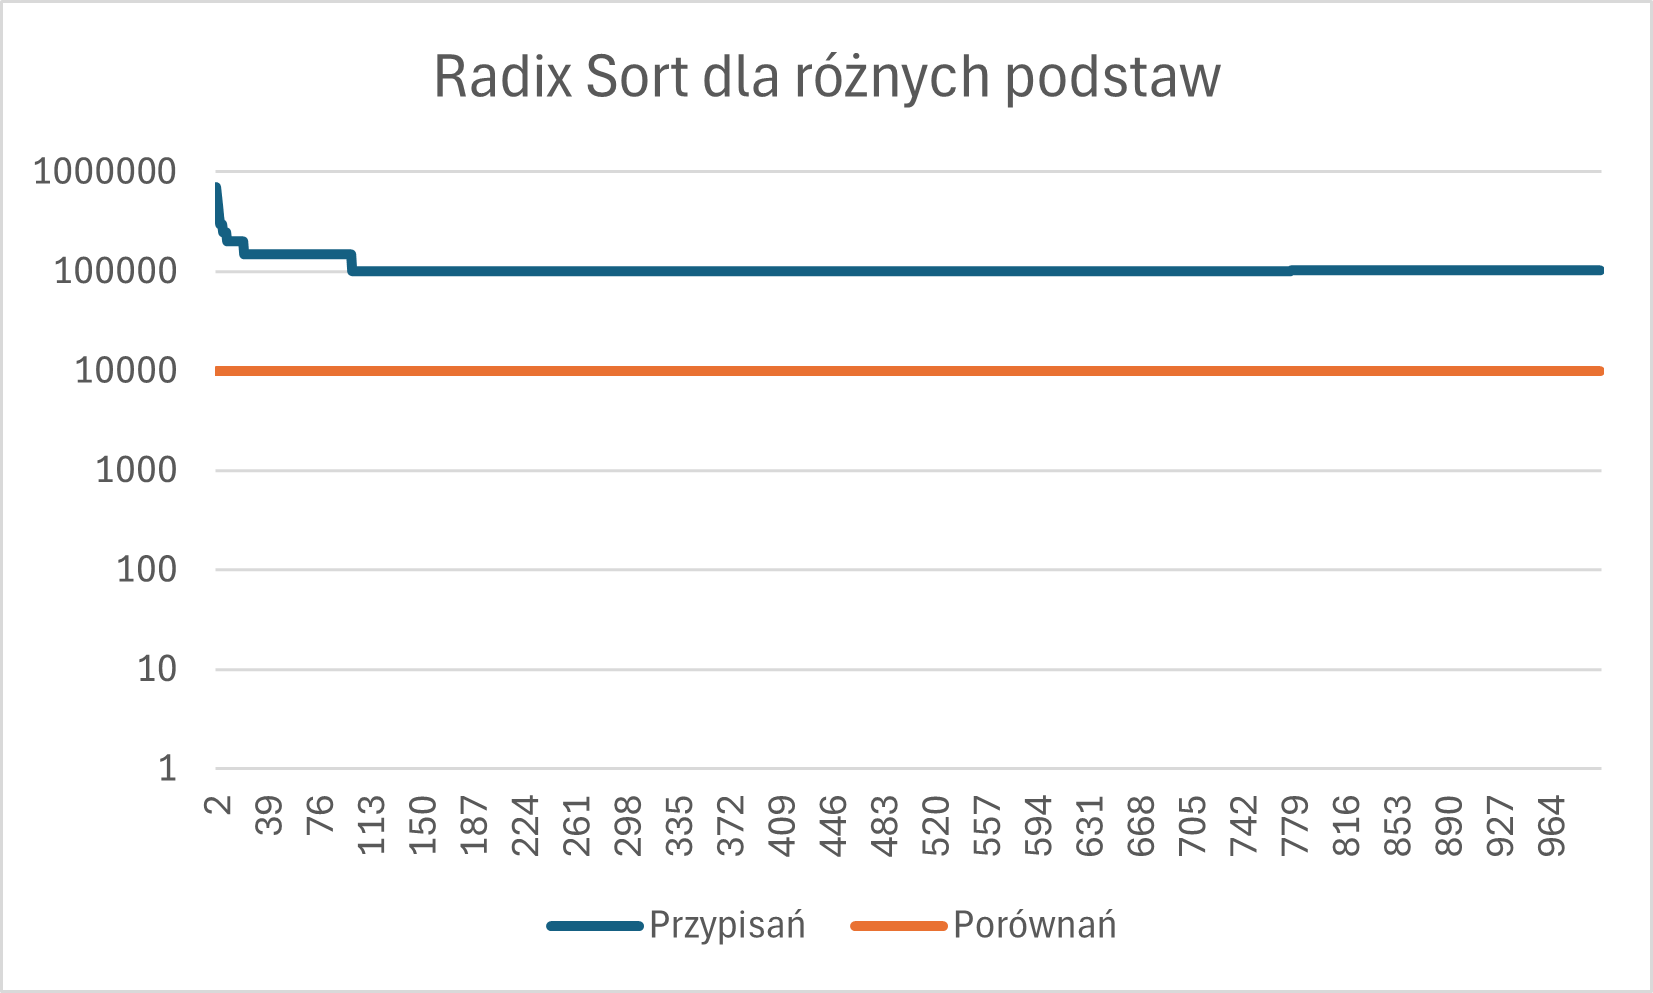
\includegraphics[width=1\textwidth]{RadixSort.png}
\end{center}

Dla zmniejszenia ilości przypisań, które musi wykonać Radix Sort, korzystne jest używanie systemów liczbowych składających się z wielu cyfr. Można zauważyć, że gdy liczba cyfr systemu rośnie, liczba przypisań spada istotnie w pewnych odstępach, co daje wizualne "schodki" na wykresie.

\begin{center}
\begin{tabular}{|c|c|}
 \hline
 d & Liczba przypisań \\ 
 \hline
 5 & 300030 \\
 6 & 300036 \\
 7 & 250036 \\
 8 & 250041 \\
 9 & 250046 \\
 10 & 200042 \\
 11 & 200046 \\
 \hline
\end{tabular}

\vspace{0.5cm}

\begin{tabular}{|c|c|}
 \hline
 d & Liczba przypisań \\ 
 \hline
 20 & 200082 \\
 21 & 200086 \\
 22 & 150069 \\
 23 & 150072 \\
 \hline
\end{tabular}

\vspace{0.5cm}

\begin{tabular}{|c|c|}
 \hline
 d & Liczba przypisań \\ 
 \hline
 98 & 150297 \\
 99 & 150300 \\
 100 & 100204 \\
 101 & 100206 \\
 \hline
\end{tabular}
\end{center}

\subsection{Quick Sort kontra Bucket Sort}

\begin{center}
    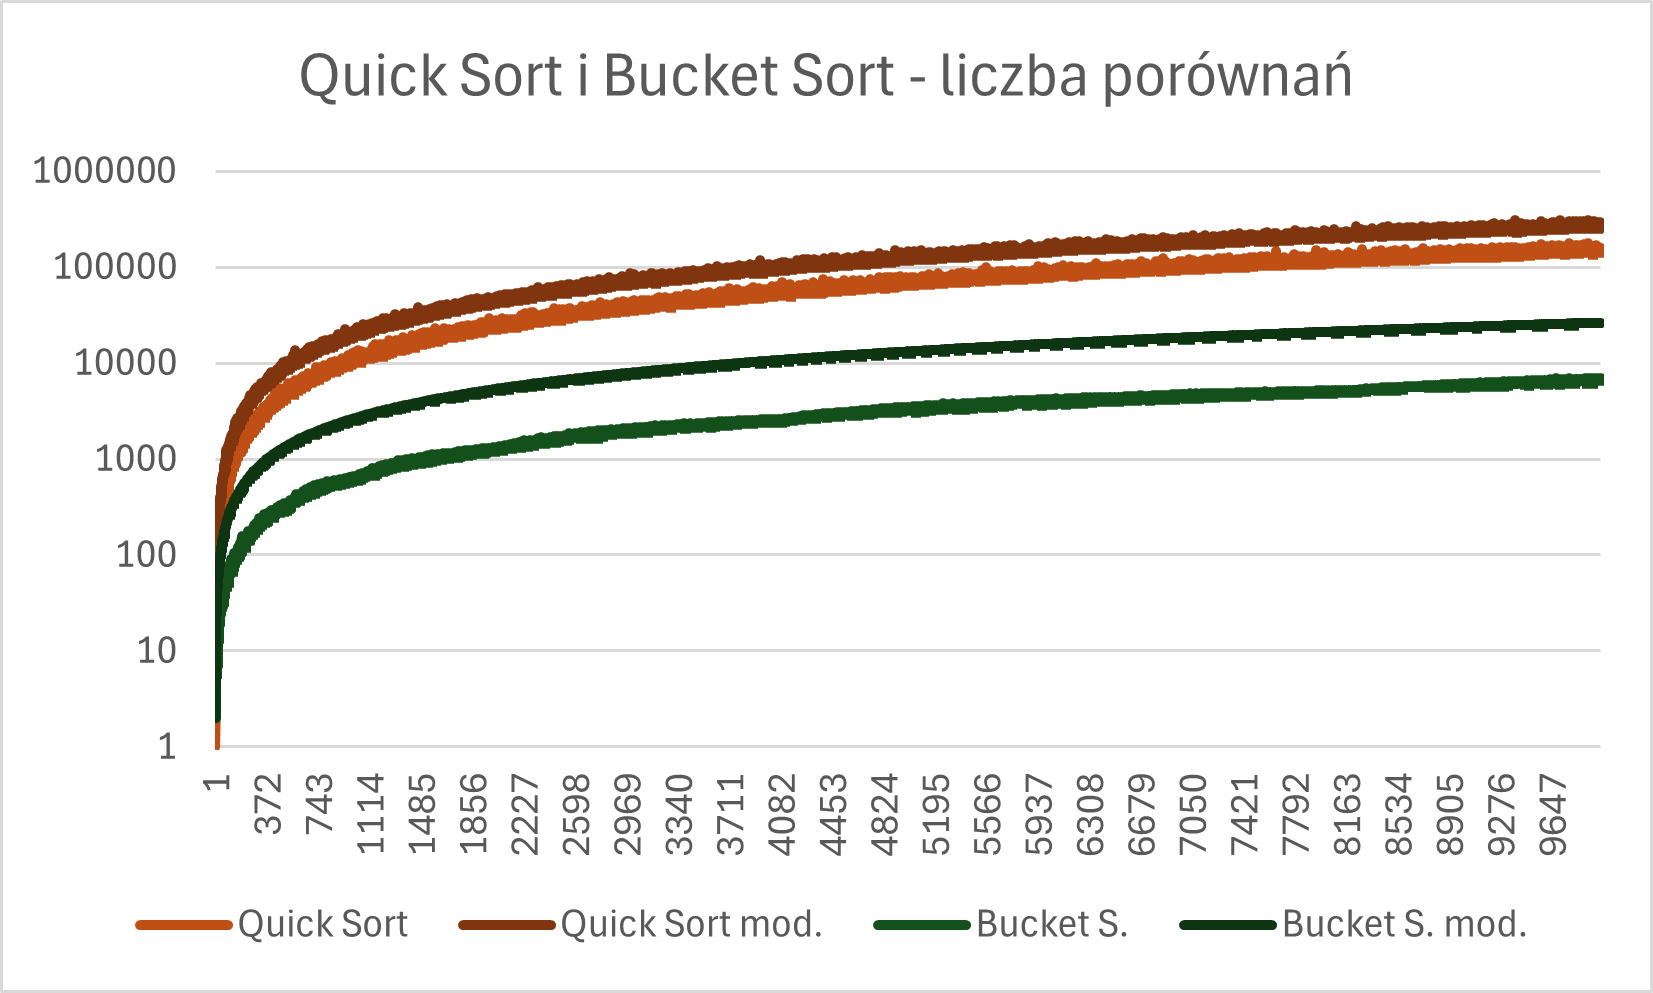
\includegraphics[width=1\textwidth]{QuickBucketPor.png}
\end{center}

\begin{center}
Liczba porównań dla danych różnych rozmiarów: 
\begin{tabular}{|c|c|c|c|c|}
 \hline
 n & Quick Sort & Quick Sort mod. & Bucket Sort & Bucket Sort mod. \\ 
 \hline
 10 & 25 & 66 & 5 & 23\\
 100 & 690 & 1285 & 60 & 263 \\
 1000 & 11266 & 20161 & 638 & 2618 \\
 10000 & 156495 & 283309 & 6953 & 26352 \\
 \hline
\end{tabular}
\end{center}

\begin{center}
    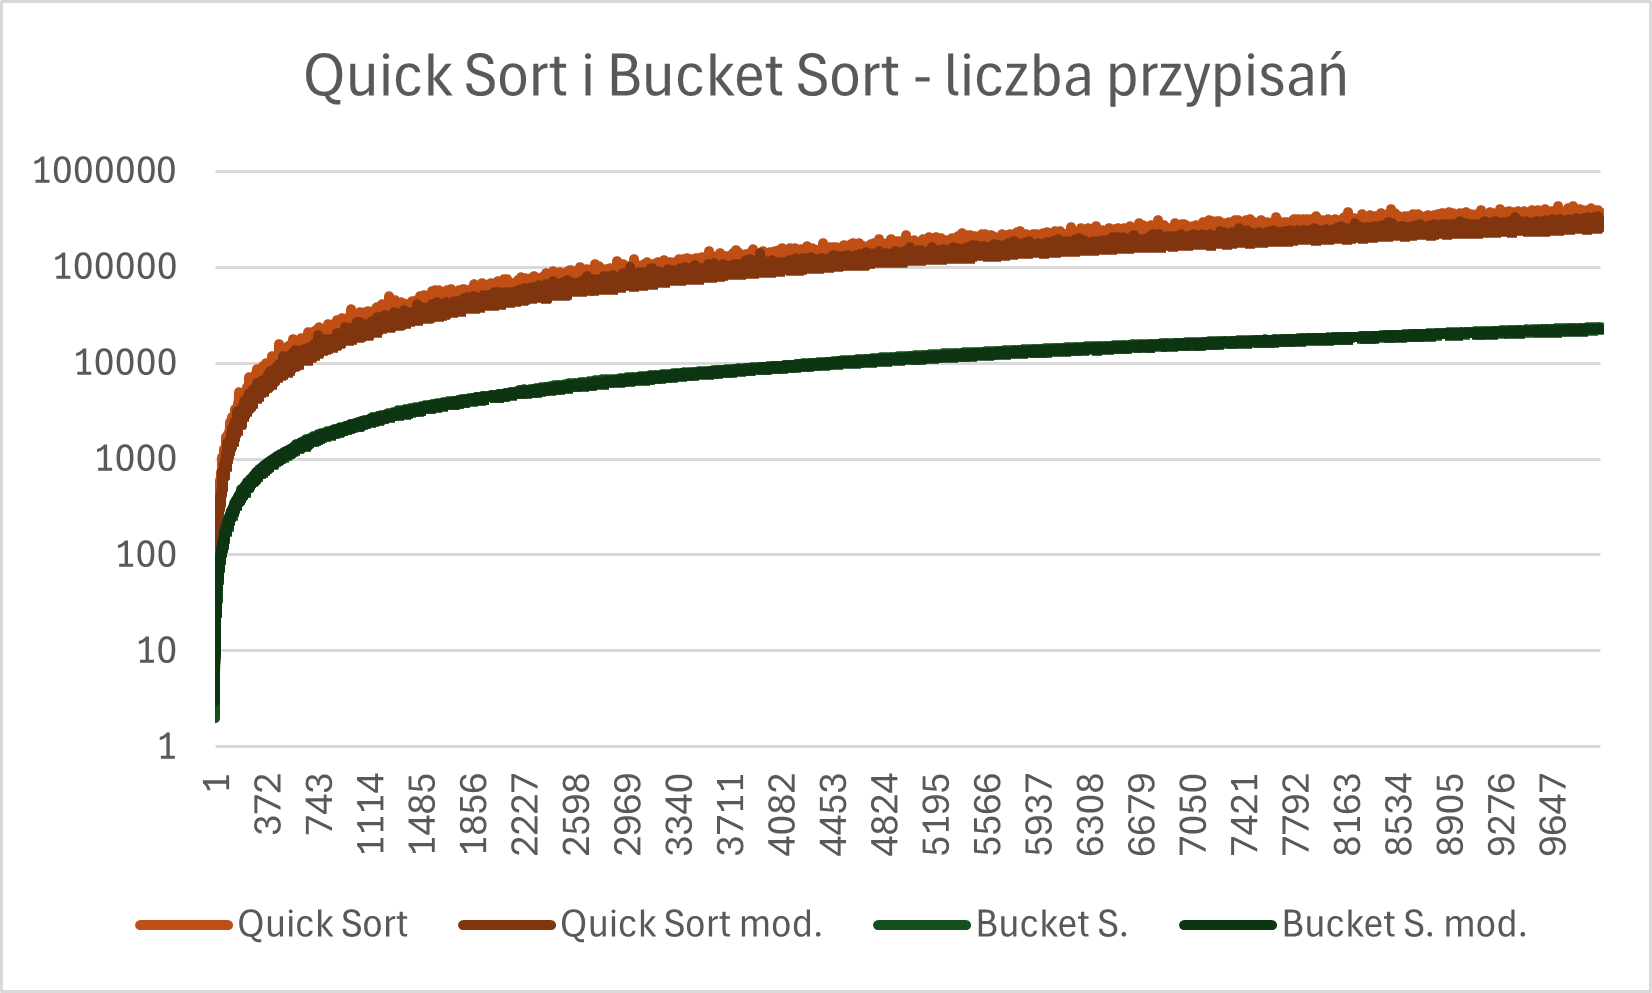
\includegraphics[width=1\textwidth]{QuickBucketPrzyp.png}
\end{center}

\begin{center}
Liczba przypisań dla danych różnych rozmiarów: 
\begin{tabular}{|c|c|c|c|c|}
 \hline
 n & Quick Sort & Quick Sort mod. & Bucket Sort & Bucket Sort mod. \\ 
 \hline
 10 & 82 & 49 & 20 & 24 \\
 100 & 1655 & 1236 & 220 & 236 \\
 1000 & 26761 & 20024 & 2272 & 2251 \\
 10000 & 363352 & 284213 & 23601 & 22727 \\
 \hline
\end{tabular}
\end{center}

\section{Wnioski}

Radix Sort działa bardziej efektywnie, gdy podstawa jest większa. Pozwala to zredukować liczbę iteracji dla kolejnych, bardziej znaczących cyfr. Należy jednak pamiętać, że wzrost podstawy powoduje większe wykorzystanie pamięci.

Na podstawie danych, Quick Sort wykazuje znacznie większą liczbę porównań i przypisań niż Bucket Sort. Modyfikacja zwiększyła liczbę porównań dla obu algorytmów, w przypadku Bucket Sort bardziej znacznie. Zmniejszyła liczbę przypisań w przypadku Quick Sort, dla Bucket Sort różnica jest zaniedbywalna (dla badanych rozmiarów tablicy).

\end{document}
